\paragraph{Retourneren}

\emph{Retourneren} is een ander woord voor \emph{teruggeven}. Het is mogelijk voor functies om een waarde terug te geven naar vanwaar de functie wordt uitgevoerd. Dit doe je met het commando \texttt{return}. De waarde die hier teruggegeven wordt noemen we ook wel het \emph{resultaat} van de functie. Het resultaat van de functie vervangt als het ware de functieaanroep zelf. Dit werkt net als het gebruik van variabelen; die worden vervangen door hun waardes.

\paragraph{Types}
Helemaal in het begin van dit hoofdstuk lieten we het volgende zien:

\begin{verbatim}
<type> <naam van functie>():
  <inhoud van functie>
\end{verbatim}

Tot nog toe hebben we alleen \texttt{void} in de plaats van \texttt{<type>} gebruikt. \texttt{void} staat voor \texttt{niets} en dit betekent dat onze functie niets teruggeeft. Dan hoef je dus ook geen \texttt{return} commando te geven. Als je wel iets wil teruggeven moet je het specifieke \texttt{type} aanduiden. In onze voorbeelden zullen we alleen de types \texttt{int}, \texttt{float}, en \texttt{string} gebruiken.

% \begin{figure}[h]
% \begin{subfigure}[b]{.3\linewidth}
% \begin{verbatim}
% int das(x):
%   return x / 4
% print(das(12))
% \end{verbatim}
% \end{subfigure}
% \begin{subfigure}[b]{.3\linewidth}
% \begin{verbatim}
% float cod():
%   return 12.0 / 4.0
% print(plo())
% \end{verbatim}
% \end{subfigure}
% \begin{subfigure}[b]{.3\linewidth}
% \begin{verbatim}
% str plo():
%   return "drie"
% print(plo())
% \end{verbatim}
% \end{subfigure}
% \end{figure}
%
% Deze stukken code printen dan:
% \begin{figure}[h]
% \begin{subfigure}[b]{.3\linewidth}
% \begin{verbatim}
% 3
% \end{verbatim}
% \end{subfigure}
% \begin{subfigure}[b]{.3\linewidth}
% \begin{verbatim}
% 3.0
% \end{verbatim}
% \end{subfigure}
% \begin{subfigure}[b]{.3\linewidth}
% \begin{verbatim}
% drie
% \end{verbatim}
% \end{subfigure}
% \end{figure}
%
% Je kan ook het resultaat van de functie opslaan in een variabele:
%
% \begin{verbatim}
% int tok(bat):
%   return bat / 2
% pet = tok(8)
% print(pet)
% print(tok(pet))
% \end{verbatim}

% Dit zou het volgende uitprinten:
%
% \begin{verbatim}
% 4
% 2
% \end{verbatim}

\paragraph{Traceren}

Functies die iets uitrekenen traceren we op vrijwel dezelfde manier als voorheen. Daar komt bij dat er iets \emph{terug}gaat van de functie naar de startregel. In het volgende voorbeeld zie je dat de functie het getal 3 uitrekent en \texttt{return}t. Dit kunnen we uiteindelijk invullen in de \texttt{print}.

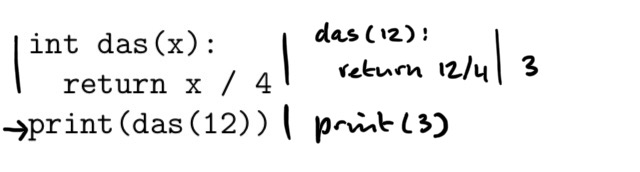
\includegraphics[width=.7\textwidth]{6-trace-returns.jpeg}
